\documentclass[vietnamese]{vlththesis}
\usepackage{tikz, amsmath}
\usetikzlibrary{calc}


\graphicspath{ {image/} }
\addbibresource{bibbi.bib}
\makenoidxglossaries

\newacronym{lppl}{LPPL}{LaTeX Project Public License}
\newacronym{tex}{\TeX}{Tau Epsilon Chi}
\newacronym{wysiwyg}{WYSIWYG}{What you see is what you get}
\newacronym{ctan}{CTAN}{Comprehensive \TeX\ Archive Network}
\newacronym{ams}{AMS}{American Mathematical Society}
\newacronym{isbn}{ISBN}{International Standard Book Number}
\newacronym{lof}{LoF}{List of Figures}
\newacronym{lot}{LoT}{List of Tables}
\newacronym{toc}{ToC}{Table of Contents}

\title{GIẢI TÍCH SỐ TÍCH PHÂN MONTE CARLO NHIỀU LỚP BẰNG GIEO ĐIỂM QUAN TRỌNG}
\author{Huỳnh Thị Hạ Vy \\& }
\supervisorName{TS. Nguyễn Chí Linh}

\makeatletter
\newcommand{\printtitlepage}{
\thispagestyle{empty}
	\begin{center}
	{\bfseries\parskip=0pt
	
	\theGroup
	\vspace*{0.1cm}
	
	\theUniversity
	\vspace*{0.1cm}
	
	\theFaculty
	\vspace*{0.1cm}
	
	\theDepartment\\
	\vspace*{0.1cm}
	------------------oOo------------------
	}
	\vspace*{1cm}
	
	{\bfseries
	\large
	\theReport}
	
	\vspace*{2cm plus 1cm minus 0.5cm}
	
	\iftoggle{viet}
	{\begin{flushleft}
		\textsl{\Large\underline{Đề tài:}}
	\end{flushleft}}
	{~}
	{\huge\bfseries
		\textcolor{cstred}{\@title}\par	
	}
	\end{center}
	
	\vspace*{2cm plus 1 cm minus 0.5cm}
	
	\hfill
	{\bfseries\large
	\iftoggle{viet}{%
	\begin{tabular}{r l}
	\underline{SVTH}: & \@author\\
	\underline{CBHD}: & \thesupervisorName\\
	\end{tabular}%
	}{%
	\begin{tabular}{r l}
	\underline{Student}: & \@author\\
	\underline{Supervisor}: & \thesupervisorName\\
	\end{tabular}%
	}}
	
	\vfill
	\begin{center}
	-----------------------------------------\\
	\bfseries
	\thePlace\ - \theDate
	\end{center}
	\clearpage


}

\makeatother


\begin{document}
\begin{titlepage}

\begin{tikzpicture}[remember picture, overlay]
  \draw[line width = 2pt] ($(current page.north west) + (1.1in,-1.1in)$) rectangle ($(current page.south east) + (-0.5in,0.9in)$);
  \draw[line width = 2pt] ($(current page.north west) + (1.2in,-1.2in)$) rectangle ($(current page.south east) + (-0.6in,1in)$);
\end{tikzpicture}
\makeatletter
\printtitlepage
\makeatother
\end{titlepage}

\printcoverpage
\acknowledgements{Lorem ipsum dolor sit amet, consectetur adipiscing elit. Maecenas volutpat ligula sed nunc porttitor efficitur. Fusce tincidunt semper efficitur. Quisque et ullamcorper eros, et blandit nibh. Aliquam tempus laoreet tellus vitae ullamcorper. Etiam ut dui et est elementum rutrum eu at ligula. Vivamus porttitor neque eget massa lacinia, eget placerat felis ullamcorper. Nullam est mi, accumsan sit amet lacus vitae, eleifend bibendum tortor.\par
Sed tincidunt gravida elit ornare suscipit. Vestibulum vitae fringilla orci. Nullam facilisis pellentesque tincidunt. Nullam congue ex id tempus condimentum. Nunc vulputate bibendum enim, eu condimentum ipsum facilisis sit amet. Curabitur iaculis venenatis odio, sed eleifend risus iaculis eget. Duis vel neque ligula. Nunc vehicula dapibus quam id efficitur. Sed elementum nisl felis, ut tincidunt mi vehicula ut. Aenean bibendum porta risus, sed tincidunt justo molestie in. Mauris dapibus ligula vitae lacus ultrices faucibus. Etiam posuere arcu non libero maximus, vel tempus enim dignissim.\par 
Lorem ipsum dolor sit amet, consectetur adipiscing elit. Maecenas volutpat ligula sed nunc porttitor efficitur. Fusce tincidunt semper efficitur. Quisque et ullamcorper eros, et blandit nibh. Aliquam tempus laoreet tellus vitae ullamcorper. Etiam ut dui et est elementum rutrum eu at ligula. Vivamus porttitor neque eget massa lacinia, eget placerat felis ullamcorper. Nullam est mi, accumsan sit amet lacus vitae, eleifend bibendum tortor.\par
Lorem ipsum dolor sit amet, consectetur adipiscing elit. Maecenas volutpat ligula sed nunc porttitor efficitur. Fusce tincidunt semper efficitur. Quisque et ullamcorper eros, et blandit nibh. Aliquam tempus laoreet tellus vitae ullamcorper. Etiam ut dui et est elementum rutrum eu at ligula. Vivamus porttitor neque eget massa lacinia, eget placerat felis ullamcorper. Nullam est mi, accumsan sit amet lacus vitae, eleifend bibendum tortor.\par}
\printfrontmatter

\startintroduction
Lorem ipsum dolor sit amet, consectetur adipiscing elit. Maecenas volutpat ligula sed nunc porttitor efficitur. Fusce tincidunt semper efficitur. Quisque et ullamcorper eros, et blandit nibh. Aliquam tempus laoreet tellus vitae ullamcorper. Etiam ut dui et est elementum rutrum eu at ligula. Vivamus porttitor neque eget massa lacinia, eget placerat felis ullamcorper. Nullam est mi, accumsan sit amet lacus vitae, eleifend bibendum tortor.\par
Sed tincidunt gravida elit ornare suscipit. Vestibulum vitae fringilla orci. Nullam facilisis pellentesque tincidunt. Nullam congue ex id tempus condimentum. Nunc vulputate bibendum enim, eu condimentum ipsum facilisis sit amet. Curabitur iaculis venenatis odio, sed eleifend risus iaculis eget. Duis vel neque ligula. Nunc vehicula dapibus quam id efficitur. Sed elementum nisl felis, ut tincidunt mi vehicula ut. Aenean bibendum porta risus, sed tincidunt justo molestie in. Mauris dapibus ligula vitae lacus ultrices faucibus. Etiam posuere arcu non libero maximus, vel tempus enim dignissim.\par 
\fancyhead[L]{\slshape\nouppercase{\chaptertitlename\ \thechapter}}
\chapter{Kiến thức cơ sở xác suất và thống kê}\label{ch:1}
\section{Biến ngẫu nhiên và xác suất}\label{sec:1.1}
Biến ngẫu nhiên là một hàm ánh xạ với đặc điểm nó gán một giá trị bằng số cho kết quả đầu ra của một phép thử ngẫu nhiên.\cite{thongke}
\begin{align}
    \textbf{x}(\omega)=\textit{x}
\end{align}
với $\omega$ là đại diện cho đầu ra của một thực nghiệm, \textit{x} là một số thực (hay sự kiện), \textbf{x} là hàm ánh xạ (hay biến ngẫu nhiên).  
Tính ngẫu nhiên được thể hiện ở tham số đầu vào $\omega$. Điều này dẫn đến đầu ra của hàm là ngẫu nhiên.\\
Đây chưa phải là định nghĩa đầy đủ của một biến ngẫu nhiên. Khái niệm khác liên quan đến định nghĩa của một biến ngẫu nhiên là khái niệm xác suất. \\
Xét một số thí dụ sau:
\begin{itemize}
    \item Gieo một đồng xu trên mặt phẳng, đây là một phép thử. Kết quả có thể xảy ra là \textit{Xuất hiện mặt sấp} hoặc \textit{Xuất hiện mặt ngửa}. Như vậy xác suất cho các khả năng \textit{Xuất hiện mặt sấp} và \textit{Xuất hiện mặt ngửa} lần lượt là 
	$ \frac{1}{2} $ và $ \frac{1}{2} $
	\begin{figure}[H]
		\centering
		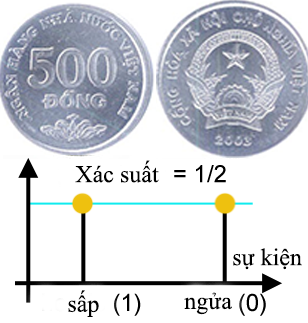
\includegraphics[width=0.4\textwidth]{coin.png}
		\caption{Các sự kiện có thể xuất hiện khi gieo đồng xu}
	   \end{figure}
    \item Gieo một con súc sắc, đây là một phép thử. Kết quả có thể xảy ra là "Xuất hiện mặt k chấm" tương ứng với k = 1,2,3,..,6. Xác suất cho mỗi sự kiện "Xuất hiện k chấm" đều là $ \frac{1}{6} $.
    \begin{figure}[H]
		\centering
		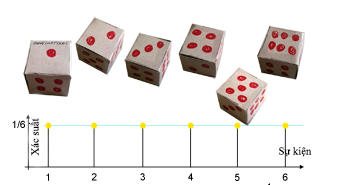
\includegraphics[width=0.6\textwidth]{xucxac.png}
		\caption{Các sự kiện có thể xuất hiện khi gieo súc sắc}
	   \end{figure}
\end{itemize}
Tổng quát, nếu một phép thử tạo ra n sự kiện khác nhau và khả năng xảy ra như nhau thì xác suất của mỗi sự kiện là $ \frac{1}{n} $
chúng ta có thể nói rằng nếu kết quả của một quá trình nào đó phải là một trong n kết quả khác nhau. 
\par
\section{Phân phối xác suất}\label{sec:1.2}
Phân phối xác suất xác định xác suất cho từng sự kiện có thể xảy ra của một phép thử ngẫu nhiên. Hàm phân phối xác suất của biến ngẫu nhiên \textbf{x} được xác định như sau:
\begin{align}
	\textbf{F}(x)=\textbf{P}(\textbf{x}\leq\textit{x})=\textbf{P}\left\{{\omega\in\Omega:\textbf{x}(\Omega)\leq\textit{x}} \right\}
\end{align}
với mọi $\textit{x}\in\textbf{R}$ được gọi là hàm phân phối xác suất của biến ngẫu nhiên $\textbf{x}$.

Đặc trưng của hàm phân phối xác suất hay gọi là hàm phân phối tích luỹ (CDF)
là lấy xác suất các biến ngẫu nhiên bên trái của một giá trị \textbf{x} bất kì nào đó.
Hàm này có đặc điểm là một hàm không giảm, tức là nếu $\textit{a}<\textit{b}$
thì $\textbf{F}(a)\leq\textbf{F}(b)$ vì sự kiện $\textit{b}$ đã bao gồm cả sự kiện $\textit{a}$ rồi.
\par
\subsection{Hàm khối xác suất của biến rời rạc}\label{subsec:1.2.1}
Hàm xác xuất để xác định xác suất tại mỗi giá trị \textbf{x} nào đó trong miền giá trị là bao nhiêu.
Hàm xác xuất như vậy được gọi là hàm khối xác suất (PMF) Đối với các biến ngẫu nhiên rời rạc. 
Giả sử miền giá trị của $\textbf{x}$ là $\textbf{D}$, tức $\textbf{x}$:$\bf\Omega\mapsto$$\textbf{D}$ thì hàm khối xác suất được xác định như sau: 
\begin{equation}
	\textit{p}(x)=\textit{p}\textit{X}(\textit{x})=
	\begin{cases}
	\textbf{P}(\textbf{x}=\textit{x}) &if \textit{x}\in\textbf{D}\\
	0 &if \textit{x}\notin\textbf{D}
	\end{cases}
\end{equation}
Như vậy ta có thể thấy rằng hàm khối xác suất thực chất cũng là một xác suất nên nó mang đầy đủ tất cả các tính chất của xác suất như:
\begin{itemize}
	\item 0$\leq\textit{p}(x)\leq$1
	\item $\sum_{x_i\in\textbf{D}}\textit{p}(x_{i})=$1
\end{itemize}
\par
\subsection{Hàm mật độ xác suất của biến liên tục}\label{subsec:1.2.2}
Hàm mật độ xác suất (PDF - Probability Density Function) đối với các biến ngẫu nhiên liên tục, dùng để ước lượng độ tập trung xác suất tại lân cận điểm nào đó.
Hàm mật độ xác suất \textit{f}(\textit{x}) tại điểm \textit{x} được xác định bằng cách lấy đạo hàm của hàm phân phối tích lũy \textbf{F}(\textit{x}) tại điểm đó:
\begin{align}
	\textit{f}(x)=\textbf{F}'(x)
\end{align}
Như vậy thì nơi nào \textit{f}(\textit{x}) càng lớn thì ở đó mức độ tập xác suất càng cao. 
Từ đây ta cũng có thể biểu diễn hàm phân phối tích luỹ như sau: 
\begin{align}
	\textbf{F}(x)=\int_{-\infty}^{x}\textit{f}(t)dt
\end{align}
Xác suất trong 1 khoảng ($\alpha$,$\beta$) cũng có thể được tính bằng hàm mật độ xác suất: 
\begin{align}
	\textbf{F}(x)=\int_{\alpha}^{\beta}\textit{f}(x)dx
\end{align}
Hàm mật độ xác suất cũng có 2 tính chất như xác suất như sau:
\begin{itemize}
	\item Không âm: $\textit{f}(x)\geq$0, $\forall(x)\in\textbf{R}$
	\item Tổng toàn miền bằng 1: $\int_{-\infty}^{\infty}\textit{f}(x)\textit{dx}$=1
\end{itemize}
\par
\section{Kỳ vọng và phương sai}\label{sec:1.3}
Giá trị kỳ vọng của X là tổng “sự kiện” nhân với xác suất của sự kiện đó. Như đã nhắc đến phần $ \ref{sec:1.2} $, 
xác suất được tính theo hàm PMF cho biến ngẫu nhiên rời rạc và hàm PDF cho biến ngẫu nhiên liên tục. 
Hay nói cách khác giá trị kỳ vọng là giá trị trung bình có trọng số.
\begin{align}
	\textbf{E}[\textbf{x}]=\sum_{i=0}^{N-1}{X_ipmf(X_i)}
\end{align}
Trong đó N là số “\textit{sự kiện}” có thể xảy ra của một biến ngẫu nhiên rời rạc $\textbf{x}$. 
Để mở rộng cho biến ngẫu nhiên liên tục $\textbf{x}$: 
\begin{align}
	\textbf{E}[\textbf{x}]=\int_{-\infty}^{\infty}{\textbf{x}pdf(\textbf{x})}
\end{align}
Giả sử $\textbf{x}$ là một biến ngẫu nhiên có tập giá trị sau {1, 2, 3, 4, 5, 6} và $\textbf{F}[\textbf{x}]=(\textbf{x}-3)^2$. Chú ý rằng  $\textbf{x}$ là biến ngẫu nhiên thì $\textbf{E}[\textbf{x}]$ cũng là một biến ngẫu nhiên.
Như vậy
\begin{itemize}
	\centering
	\item $\textbf{x}=1,\textbf{F}(1)=(1-3)^2=4$
	\item $\textbf{x}=2,\textbf{F}(2)=(2-3)^2=1$
	\item $\textbf{x}=3,\textbf{F}(3)=(3-3)^2=0$
	\item $\textbf{x}=4,\textbf{F}(4)=(4-3)^2=1$
	\item $\textbf{x}=5,\textbf{F}(5)=(5-3)^2=4$
	\item $\textbf{x}=6,\textbf{F}(6)=(6-3)^2=9$
\end{itemize}
Nhận thấy, xác suất của một kết quả $\textbf{Y}$ từ $\textbf{F}[\textbf{x}]$ bằng tổng xác suất của bất kỳ X nào thỏa $\textbf{F}[\textbf{x}]=\textbf{Y}$.

\begin{itemize}
	\centering
	\item $\textbf{P}(\textbf{F}(0))=\frac{1}{6}$
	\item $\textbf{P}(\textbf{F}(1))=\frac{1}{6}+\frac{1}{6}=\frac{2}{6}$
	\item $\textbf{P}(\textbf{F}(4))=\frac{1}{6}+\frac{1}{6}=\frac{2}{6}$
	\item $\textbf{P}(\textbf{F}(9))=\frac{1}{6}$
\end{itemize}

Trong toán học có hai phương pháp để tính giá trị kỳ vọng của $\textbf{F}[\textbf{x}]$ 
\begin{itemize}
	\item Phương pháp 1: Nếu phân phối xác suất của $\textbf{F}[\textbf{x}]$ đã biết trước, thì giá trị kỳ vọng được tính như sau:
	\begin{align}
		\textbf{E}[\textbf{F}[\textbf{x}]]=\textbf{E}[\textbf{Y}]=\sum{Y_i\textbf{P}(Y_i)}
	\end{align}
	\item Phương pháp 2: Nếu phân phối xác suất của $\textbf{F}[\textbf{x}]$ chưa biết trước, thì giá trị kỳ vọng được tính như sau: 
	Đối với biến ngẫu nhiên rời rạc
	\begin{align}
		\textbf{E}[\textbf{F}(\textbf{x})]=\sum{\textbf{F}(\textbf{x})\textbf{P}(\textbf{x})}
	\end{align}
	Đối với biến ngẫu nhiên liên tục
	\begin{align}
		\textbf{E}[\textbf{F}(\textbf{x})]=\int{\textbf{F}(\textbf{x})\textbf{P}(\textbf{x})d\textbf{x}}
	\end{align}
\end{itemize}
Phương pháp 2 đóng vai trò quan trọng trong phương pháp Monte Carlo. 
Bởi vì hàm phân phối xác xuất $\textbf{F}(\textbf{x})$ có thể không được biết trước.
Phương sai được xác định như sau
\begin{align}
	\sigma^2[\textbf{Y}]=E[(\textbf{Y}-\textbf{E}[\textbf{Y}])^2]
\end{align}
trong đó $\sigma$, độ lệch chuẩn, là căn bậc hai của phương sai. 
Từ những định nghĩa này, nó là dễ dàng cho thấy rằng với bất kỳ hằng số a
\begin{align}
	\textbf{E}[a\textbf{Y}]=a\textbf{E}[\textbf{Y}]
\end{align}
\begin{align}
	\sigma^2[a\textbf{Y}]=a^2\sigma^2[\textbf{Y}]
\end{align}
Hơn nữa, giá trị kỳ vọng của một tổng các biến ngẫu nhiên Yi là tổng giá trị kỳ vọng của Yi:
\begin{align}
	E\left[\sum_i{Y_i}\right]=\sum_i{E[Y_i]}
\end{align}
Từ các tính chất này, có thể rút ra biểu thức đơn giản hơn cho phương sai:
\begin{align}
	\sigma^2[\textbf{Y}]=\textbf{E}[\textbf{Y}^2]-\textbf{E}[\textbf{Y}]^2
\end{align}
Ngoài ra, nếu các biến ngẫu nhiên độc lập thì:
\begin{align}
	\sigma^2\left[\sum_i{Y_i}\right]=\sum_i{\sigma^2[Y_i]}\label{ct1.17}
\end{align}

\chapter{Chapter 2 Title}
Lorem ipsum dolor sit amet, consectetur adipiscing elit. Maecenas volutpat ligula sed nunc porttitor efficitur. Fusce tincidunt semper efficitur. Quisque et ullamcorper eros, et blandit nibh. Aliquam tempus laoreet tellus vitae ullamcorper. Etiam ut dui et est elementum rutrum eu at ligula. Vivamus porttitor neque eget massa lacinia, eget placerat felis ullamcorper. Nullam est mi, accumsan sit amet lacus vitae, eleifend bibendum tortor. \par
Sed tincidunt gravida elit ornare suscipit. Vestibulum vitae fringilla orci. Nullam facilisis pellentesque tincidunt. Nullam congue ex id tempus condimentum. Nunc vulputate bibendum enim, eu condimentum ipsum facilisis sit amet. Curabitur iaculis venenatis odio, sed eleifend risus iaculis eget. Duis vel neque ligula. Nunc vehicula dapibus quam id efficitur. Sed elementum nisl felis, ut tincidunt mi vehicula ut. Aenean bibendum porta risus, sed tincidunt justo molestie in. Mauris dapibus ligula vitae lacus ultrices faucibus. Etiam posuere arcu non libero maximus, vel tempus enim dignissim.\par 

\section{2.1 Title}
Sed tincidunt gravida elit ornare suscipit. Vestibulum vitae fringilla orci. Nullam facilisis pellentesque tincidunt. Nullam congue ex id tempus condimentum. Nunc vulputate bibendum enim, eu condimentum ipsum facilisis sit amet. Curabitur iaculis venenatis odio, sed eleifend risus iaculis eget. Duis vel neque ligula. Nunc vehicula dapibus quam id efficitur. Sed elementum nisl felis, ut tincidunt mi vehicula ut. Aenean bibendum porta risus, sed tincidunt justo molestie in. Mauris dapibus ligula vitae lacus ultrices faucibus. Etiam posuere arcu non libero maximus, vel tempus enim dignissim. \par
Sed tincidunt gravida elit ornare suscipit. Vestibulum vitae fringilla orci. Nullam facilisis pellentesque tincidunt. Nullam congue ex id tempus condimentum. Nunc vulputate bibendum enim, eu condimentum ipsum facilisis sit amet. Curabitur iaculis venenatis odio, sed eleifend risus iaculis eget. Duis vel neque ligula. Nunc vehicula dapibus quam id efficitur. Sed elementum nisl felis, ut tincidunt mi vehicula ut. Aenean bibendum porta risus, sed tincidunt justo molestie in. Mauris dapibus ligula vitae lacus ultrices faucibus. Etiam posuere arcu non libero maximus, vel tempus enim dignissim. \par
Sed tincidunt gravida elit ornare suscipit. Vestibulum vitae fringilla orci. Nullam facilisis pellentesque tincidunt. Nullam congue ex id tempus condimentum. Nunc vulputate bibendum enim, eu condimentum ipsum facilisis sit amet. Curabitur iaculis venenatis odio, sed eleifend risus iaculis eget. Duis vel neque ligula. Nunc vehicula dapibus quam id efficitur. Sed elementum nisl felis, ut tincidunt mi vehicula ut. Aenean bibendum porta risus, sed tincidunt justo molestie in. Mauris dapibus ligula vitae lacus ultrices faucibus. Etiam posuere arcu non libero maximus, vel tempus enim dignissim. \par
Sed tincidunt gravida elit ornare suscipit. Vestibulum vitae fringilla orci. Nullam facilisis pellentesque tincidunt. Nullam congue ex id tempus condimentum. Nunc vulputate bibendum enim, eu condimentum ipsum facilisis sit amet. Curabitur iaculis venenatis odio, sed eleifend risus iaculis eget. Duis vel neque ligula. Nunc vehicula dapibus quam id efficitur. Sed elementum nisl felis, ut tincidunt mi vehicula ut. Aenean bibendum porta risus, sed tincidunt justo molestie in. Mauris dapibus ligula vitae lacus ultrices faucibus. Etiam posuere arcu non libero maximus, vel tempus enim dignissim. \par
Sed tincidunt gravida elit ornare suscipit. Vestibulum vitae fringilla orci. Nullam facilisis pellentesque tincidunt. Nullam congue ex id tempus condimentum. Nunc vulputate bibendum enim, eu condimentum ipsum facilisis sit amet. Curabitur iaculis venenatis odio, sed eleifend risus iaculis eget. Duis vel neque ligula. Nunc vehicula dapibus quam id efficitur. Sed elementum nisl felis, ut tincidunt mi vehicula ut. Aenean bibendum porta risus, sed tincidunt justo molestie in. Mauris dapibus ligula vitae lacus ultrices faucibus. Etiam posuere arcu non libero maximus, vel tempus enim dignissim. \par
Sed tincidunt gravida elit ornare suscipit. Vestibulum vitae fringilla orci. Nullam facilisis pellentesque tincidunt. Nullam congue ex id tempus condimentum. Nunc vulputate bibendum enim, eu condimentum ipsum facilisis sit amet. Curabitur iaculis venenatis odio, sed eleifend risus iaculis eget. Duis vel neque ligula. Nunc vehicula dapibus quam id efficitur. Sed elementum nisl felis, ut tincidunt mi vehicula ut. Aenean bibendum porta risus, sed tincidunt justo molestie in. Mauris dapibus ligula vitae lacus ultrices faucibus. Etiam posuere arcu non libero maximus, vel tempus enim dignissim. \par
Sed tincidunt gravida elit ornare suscipit. Vestibulum vitae fringilla orci. Nullam facilisis pellentesque tincidunt. Nullam congue ex id tempus condimentum. Nunc vulputate bibendum enim, eu condimentum ipsum facilisis sit amet. Curabitur iaculis venenatis odio, sed eleifend risus iaculis eget. Duis vel neque ligula. Nunc vehicula dapibus quam id efficitur. Sed elementum nisl felis, ut tincidunt mi vehicula ut. Aenean bibendum porta risus, sed tincidunt justo molestie in. Mauris dapibus ligula vitae lacus ultrices faucibus. Etiam posuere arcu non libero maximus, vel tempus enim dignissim. \par
Sed tincidunt gravida elit ornare suscipit. Vestibulum vitae fringilla orci. Nullam facilisis pellentesque tincidunt. Nullam congue ex id tempus condimentum. Nunc vulputate bibendum enim, eu condimentum ipsum facilisis sit amet. Curabitur iaculis venenatis odio, sed eleifend risus iaculis eget. Duis vel neque ligula. Nunc vehicula dapibus quam id efficitur. Sed elementum nisl felis, ut tincidunt mi vehicula ut. Aenean bibendum porta risus, sed tincidunt justo molestie in. Mauris dapibus ligula vitae lacus ultrices faucibus. Etiam posuere arcu non libero maximus, vel tempus enim dignissim. \par
Sed tincidunt gravida elit ornare suscipit. Vestibulum vitae fringilla orci. Nullam facilisis pellentesque tincidunt. Nullam congue ex id tempus condimentum. Nunc vulputate bibendum enim, eu condimentum ipsum facilisis sit amet. Curabitur iaculis venenatis odio, sed eleifend risus iaculis eget. Duis vel neque ligula. Nunc vehicula dapibus quam id efficitur. Sed elementum nisl felis, ut tincidunt mi vehicula ut. Aenean bibendum porta risus, sed tincidunt justo molestie in. Mauris dapibus ligula vitae lacus ultrices faucibus. Etiam posuere arcu non libero maximus, vel tempus enim dignissim. \par
Sed tincidunt gravida elit ornare suscipit. Vestibulum vitae fringilla orci. Nullam facilisis pellentesque tincidunt. Nullam congue ex id tempus condimentum. Nunc vulputate bibendum enim, eu condimentum ipsum facilisis sit amet. Curabitur iaculis venenatis odio, sed eleifend risus iaculis eget. Duis vel neque ligula. Nunc vehicula dapibus quam id efficitur. Sed elementum nisl felis, ut tincidunt mi vehicula ut. Aenean bibendum porta risus, sed tincidunt justo molestie in. Mauris dapibus ligula vitae lacus ultrices faucibus. Etiam posuere arcu non libero maximus, vel tempus enim dignissim. \par
Sed tincidunt gravida elit ornare suscipit. Vestibulum vitae fringilla orci. Nullam facilisis pellentesque tincidunt. Nullam congue ex id tempus condimentum. Nunc vulputate bibendum enim, eu condimentum ipsum facilisis sit amet. Curabitur iaculis venenatis odio, sed eleifend risus iaculis eget. Duis vel neque ligula. Nunc vehicula dapibus quam id efficitur. Sed elementum nisl felis, ut tincidunt mi vehicula ut. Aenean bibendum porta risus, sed tincidunt justo molestie in. Mauris dapibus ligula vitae lacus ultrices faucibus. Etiam posuere arcu non libero maximus, vel tempus enim dignissim. \par
Sed tincidunt gravida elit ornare suscipit. Vestibulum vitae fringilla orci. Nullam facilisis pellentesque tincidunt. Nullam congue ex id tempus condimentum. Nunc vulputate bibendum enim, eu condimentum ipsum facilisis sit amet. Curabitur iaculis venenatis odio, sed eleifend risus iaculis eget. Duis vel neque ligula. Nunc vehicula dapibus quam id efficitur. Sed elementum nisl felis, ut tincidunt mi vehicula ut. Aenean bibendum porta risus, sed tincidunt justo molestie in. Mauris dapibus ligula vitae lacus ultrices faucibus. Etiam posuere arcu non libero maximus, vel tempus enim dignissim. \par
Sed tincidunt gravida elit ornare suscipit. Vestibulum vitae fringilla orci. Nullam facilisis pellentesque tincidunt. Nullam congue ex id tempus condimentum. Nunc vulputate bibendum enim, eu condimentum ipsum facilisis sit amet. Curabitur iaculis venenatis odio, sed eleifend risus iaculis eget. Duis vel neque ligula. Nunc vehicula dapibus quam id efficitur. Sed elementum nisl felis, ut tincidunt mi vehicula ut. Aenean bibendum porta risus, sed tincidunt justo molestie in. Mauris dapibus ligula vitae lacus ultrices faucibus. Etiam posuere arcu non libero maximus, vel tempus enim dignissim. \par
\section{2.2 Title}
Sed tincidunt gravida elit ornare suscipit. Vestibulum vitae fringilla orci. Nullam facilisis pellentesque tincidunt. Nullam congue ex id tempus condimentum. Nunc vulputate bibendum enim, eu condimentum ipsum facilisis sit amet. Curabitur iaculis venenatis odio, sed eleifend risus iaculis eget. Duis vel neque ligula. Nunc vehicula dapibus quam id efficitur. Sed elementum nisl felis, ut tincidunt mi vehicula ut. Aenean bibendum porta risus, sed tincidunt justo molestie in. Mauris dapibus ligula vitae lacus ultrices faucibus. Etiam posuere arcu non libero maximus, vel tempus enim dignissim. \par
Sed tincidunt gravida elit ornare suscipit. Vestibulum vitae fringilla orci. Nullam facilisis pellentesque tincidunt. Nullam congue ex id tempus condimentum. Nunc vulputate bibendum enim, eu condimentum ipsum facilisis sit amet. Curabitur iaculis venenatis odio, sed eleifend risus iaculis eget. Duis vel neque ligula. Nunc vehicula dapibus quam id efficitur. Sed elementum nisl felis, ut tincidunt mi vehicula ut. Aenean bibendum porta risus, sed tincidunt justo molestie in. Mauris dapibus ligula vitae lacus ultrices faucibus. Etiam posuere arcu non libero maximus, vel tempus enim dignissim. \par
Sed tincidunt gravida elit ornare suscipit. Vestibulum vitae fringilla orci. Nullam facilisis pellentesque tincidunt. Nullam congue ex id tempus condimentum. Nunc vulputate bibendum enim, eu condimentum ipsum facilisis sit amet. Curabitur iaculis venenatis odio, sed eleifend risus iaculis eget. Duis vel neque ligula. Nunc vehicula dapibus quam id efficitur. Sed elementum nisl felis, ut tincidunt mi vehicula ut. Aenean bibendum porta risus, sed tincidunt justo molestie in. Mauris dapibus ligula vitae lacus ultrices faucibus. Etiam posuere arcu non libero maximus, vel tempus enim dignissim. \par
Sed tincidunt gravida elit ornare suscipit. Vestibulum vitae fringilla orci. Nullam facilisis pellentesque tincidunt. Nullam congue ex id tempus condimentum. Nunc vulputate bibendum enim, eu condimentum ipsum facilisis sit amet. Curabitur iaculis venenatis odio, sed eleifend risus iaculis eget. Duis vel neque ligula. Nunc vehicula dapibus quam id efficitur. Sed elementum nisl felis, ut tincidunt mi vehicula ut. Aenean bibendum porta risus, sed tincidunt justo molestie in. Mauris dapibus ligula vitae lacus ultrices faucibus. Etiam posuere arcu non libero maximus, vel tempus enim dignissim. \par
Sed tincidunt gravida elit ornare suscipit. Vestibulum vitae fringilla orci. Nullam facilisis pellentesque tincidunt. Nullam congue ex id tempus condimentum. Nunc vulputate bibendum enim, eu condimentum ipsum facilisis sit amet. Curabitur iaculis venenatis odio, sed eleifend risus iaculis eget. Duis vel neque ligula. Nunc vehicula dapibus quam id efficitur. Sed elementum nisl felis, ut tincidunt mi vehicula ut. Aenean bibendum porta risus, sed tincidunt justo molestie in. Mauris dapibus ligula vitae lacus ultrices faucibus. Etiam posuere arcu non libero maximus, vel tempus enim dignissim. \par
Sed tincidunt gravida elit ornare suscipit. Vestibulum vitae fringilla orci. Nullam facilisis pellentesque tincidunt. Nullam congue ex id tempus condimentum. Nunc vulputate bibendum enim, eu condimentum ipsum facilisis sit amet. Curabitur iaculis venenatis odio, sed eleifend risus iaculis eget. Duis vel neque ligula. Nunc vehicula dapibus quam id efficitur. Sed elementum nisl felis, ut tincidunt mi vehicula ut. Aenean bibendum porta risus, sed tincidunt justo molestie in. Mauris dapibus ligula vitae lacus ultrices faucibus. Etiam posuere arcu non libero maximus, vel tempus enim dignissim. \par
Sed tincidunt gravida elit ornare suscipit. Vestibulum vitae fringilla orci. Nullam facilisis pellentesque tincidunt. Nullam congue ex id tempus condimentum. Nunc vulputate bibendum enim, eu condimentum ipsum facilisis sit amet. Curabitur iaculis venenatis odio, sed eleifend risus iaculis eget. Duis vel neque ligula. Nunc vehicula dapibus quam id efficitur. Sed elementum nisl felis, ut tincidunt mi vehicula ut. Aenean bibendum porta risus, sed tincidunt justo molestie in. Mauris dapibus ligula vitae lacus ultrices faucibus. Etiam posuere arcu non libero maximus, vel tempus enim dignissim. \par
Sed tincidunt gravida elit ornare suscipit. Vestibulum vitae fringilla orci. Nullam facilisis pellentesque tincidunt. Nullam congue ex id tempus condimentum. Nunc vulputate bibendum enim, eu condimentum ipsum facilisis sit amet. Curabitur iaculis venenatis odio, sed eleifend risus iaculis eget. Duis vel neque ligula. Nunc vehicula dapibus quam id efficitur. Sed elementum nisl felis, ut tincidunt mi vehicula ut. Aenean bibendum porta risus, sed tincidunt justo molestie in. Mauris dapibus ligula vitae lacus ultrices faucibus. Etiam posuere arcu non libero maximus, vel tempus enim dignissim. \par
Sed tincidunt gravida elit ornare suscipit. Vestibulum vitae fringilla orci. Nullam facilisis pellentesque tincidunt. Nullam congue ex id tempus condimentum. Nunc vulputate bibendum enim, eu condimentum ipsum facilisis sit amet. Curabitur iaculis venenatis odio, sed eleifend risus iaculis eget. Duis vel neque ligula. Nunc vehicula dapibus quam id efficitur. Sed elementum nisl felis, ut tincidunt mi vehicula ut. Aenean bibendum porta risus, sed tincidunt justo molestie in. Mauris dapibus ligula vitae lacus ultrices faucibus. Etiam posuere arcu non libero maximus, vel tempus enim dignissim. \par
Sed tincidunt gravida elit ornare suscipit. Vestibulum vitae fringilla orci. Nullam facilisis pellentesque tincidunt. Nullam congue ex id tempus condimentum. Nunc vulputate bibendum enim, eu condimentum ipsum facilisis sit amet. Curabitur iaculis venenatis odio, sed eleifend risus iaculis eget. Duis vel neque ligula. Nunc vehicula dapibus quam id efficitur. Sed elementum nisl felis, ut tincidunt mi vehicula ut. Aenean bibendum porta risus, sed tincidunt justo molestie in. Mauris dapibus ligula vitae lacus ultrices faucibus. Etiam posuere arcu non libero maximus, vel tempus enim dignissim. \par
Sed tincidunt gravida elit ornare suscipit. Vestibulum vitae fringilla orci. Nullam facilisis pellentesque tincidunt. Nullam congue ex id tempus condimentum. Nunc vulputate bibendum enim, eu condimentum ipsum facilisis sit amet. Curabitur iaculis venenatis odio, sed eleifend risus iaculis eget. Duis vel neque ligula. Nunc vehicula dapibus quam id efficitur. Sed elementum nisl felis, ut tincidunt mi vehicula ut. Aenean bibendum porta risus, sed tincidunt justo molestie in. Mauris dapibus ligula vitae lacus ultrices faucibus. Etiam posuere arcu non libero maximus, vel tempus enim dignissim. \par
Sed tincidunt gravida elit ornare suscipit. Vestibulum vitae fringilla orci. Nullam facilisis pellentesque tincidunt. Nullam congue ex id tempus condimentum. Nunc vulputate bibendum enim, eu condimentum ipsum facilisis sit amet. Curabitur iaculis venenatis odio, sed eleifend risus iaculis eget. Duis vel neque ligula. Nunc vehicula dapibus quam id efficitur. Sed elementum nisl felis, ut tincidunt mi vehicula ut. Aenean bibendum porta risus, sed tincidunt justo molestie in. Mauris dapibus ligula vitae lacus ultrices faucibus. Etiam posuere arcu non libero maximus, vel tempus enim dignissim. \par

\chapter{Thuật toán Vegas}\label{ch:3}
\section{Giới thiệu}\label{sec:3.1}
Phương pháp Monte Carlo sử dụng các thuật toán để giải quyết các bài toán trên máy tính bằng cách lấy mẫu ngẫu nhiên. 
Kết quả của phương pháp Monte Carlo này càng chính xác khi số lượng mẫu càng tăng. 
Theo quy luật số lớn khi kích thước mẫu càng lớn thì tốc độ hội tụ của tích phân càng lớn. 
Nhưng khi mở rộng số chiều của tích phân thì số lượng mẫu cũng phải tăng theo. Điều này cũng làm ảnh hưởng đến tốc độ tính toán của máy tính.
Nếu cố định số lượng mẫu thì tốc độ hội tụ của tích phân sẽ giảm khi số chiều tăng lên. Nhìn chung, tốc độ hội tụ của phương pháp Monte Carlo là khá thấp.
Vì vậy, phương pháp tích phân Monte-Carlo sử dụng thuật toán Vegas sẽ giải quyết hiệu quả với các tích phân nhiều chiều.
\par
Đặc điểm thuật toán: 
\begin{enumerate}
      \item Phương sai chính xác cho tích phân thì được tính toán dễ dàng.
      \item Hàm tính tích phân không cần liên tục khi sử dụng thuật toán mới này. Đặc biệt, các hàm bước nhảy cũng không có vấn đề gì. Vì thế để tính tích phân nhiều chiều là việc đơn giản.
      \item Tốc độ hội tụ không phụ thuộc vào số chiều của tích phân.
      \item Đây là thuật toán thích nghi, nó tự động tập trung tính toán tích phân tại những vùng có tích phân quan trọng nhất.
\end{enumerate}
Đặc điểm (1) và (3) là phổ biến trong tất cả phương pháp Monte Carlo. Với (4) là một tính năng quan trọng nhất trong thuật toán này. Vấn đề chính trong tính toán các tích phân nhiều chiều là việc tăng số lượng mẫu theo cấp số nhân khi tăng số chiều. 
Do đó, mục đích chung của thuật toán để tính toán tích phân nhiều chiều là thích nghi.
\section{Tích phân Monte Carlo sử dụng thuật toán Vegas}\label{sec:3.2}
Monte Carlo thật ra là một phương pháp khá đơn giản. Nhưng 
vấn đề giảm phương sai cần được quan tâm. Để giảm phương sai, tất cả những gì có thể làm là tăng số lượng mẫu N. 
Muốn giảm phương sai xuống hai lần thì phải tăng gấp bốn lần số mẫu. Đối với các hàm tích phân nhiều chiều, 
số lượng mẫu tăng theo cấp số nhân khi số chiều tăng lên. Do đó, có nhiều phương pháp đã được nghiên cứu để giảm phương sai mà 
không cần tăng số lượng mẫu N. Như vậy, phương pháp lấy mẫu trọng và phương pháp lấy mẫu phân tầng được thuật toán Vegas sử 
dụng để giảm phương sai.\par
\subsection{Lấy mẫu trọng}\label{subsec:3.2.1}
\subsection{Lấy mẫu phân tầng}\label{subsec:3.2.2}
\subsection{Thuật toán Vegas}\label{subsec:3.2.3}

\chapter{Kết luận và hướng phát triển}\label{ch:4}


\thebackmatter
\chapter{Định nghĩa đầy đủ của câu lệnh}\label{append:A}
\lstset{escapeinside={(*}{*)}, frame=single}

Định nghĩa đầy đủ của hai câu lệnh \path|\printcoverpage| và \path|\printfrontmatter| ở phần \ref{sec:3.3.3} sẽ được nêu chi tiết ở phần này.
Như đã nói ở mục đó, \path|\printcoverpage| sử dụng các macro được định nghĩa riêng trong lớp và các câu lệnh để xây dựng trang bìa.
Dưới đây là phần định nghĩa của các macro nói trên.\par~\par
\begin{lstlisting}[firstnumber=183]
\iftoggle{viet}{%
	\def\theGroup{(*ĐẠI HỌC QUỐC GIA TP.HỒ CHÍ MINH*)}%
}{%
	\def\theGroup{Vietnam National University - Ho Chi Minh City}%
}

\iftoggle{viet}{%
	\def\theUniversity{(*TRƯỜNG ĐẠI HỌC KHOA HỌC TỰ NHIÊN*)}%
}{%
	\def\theUniversity{University of Science}%
}

\iftoggle{viet}{%
	\def\theFaculty{(*KHOA VẬT LÝ - VẬT LÝ KỸ THUẬT*)}%
}{%
	\def\theFaculty{Faculty of Physics and Engineering Physics}%
}

\iftoggle{viet}{%
	\def\theDepartment{(*CHUYÊN NGÀNH VẬT LÝ TIN HỌC*)}%
}{%
	\def\theDepartment{Department of Physics and Computer Science}%
}

\iftoggle{viet}{%
	\def\theReport{(*KHOÁ LUẬN TỐT NGHIỆP*)}%
}{%
	\def\theReport{BACHELOR THESIS}%
}

\iftoggle{viet}{%
	\def\thePlace{(*TP. HỒ CHÍ MINH*)}%
}{%
	\def\thePlace{HO CHI MINH CITY}%
}

\def\theDate{\the\year}
\end{lstlisting}

Các câu lệnh điều kiện \path|\iftoggle{viet}| dùng để kiểm tra tuỳ chọn \textbf{vietnamese}. Tiếp theo, là định nghĩa đầy đủ của \path|\printcoverpage|:\par~\par

\begin{lstlisting}[firstnumber=223]
\newcommand{\printcoverpage}{%
	\thispagestyle{empty}
	\begin{center}
	{\bfseries\parskip=0pt
	
	\theGroup
	\vspace*{0.1cm}
	
	\theUniversity
	\vspace*{0.1cm}
	
	\theFaculty
	\vspace*{0.1cm}
	
	\theDepartment\\
	\vspace*{0.1cm}
	------------------oOo------------------
	}
	\vspace*{1cm}
	
	{\bfseries
	\large
	\theReport}
	
	\vspace*{2cm plus 1cm minus 0.5cm}
	
	\iftoggle{viet}
	{\begin{flushleft}
		\textsl{\Large\underline{(*Đề tài*):}}
	\end{flushleft}}
	{~}
	{\huge\bfseries
		\@title\par	
	}
	\end{center}
	
	\vspace*{2cm plus 1 cm minus 0.5cm}
	
	\hfill
	{\bfseries\large
	\iftoggle{viet}{%
	\begin{tabular}{r l}
	\underline{SVTH}: & \@author\\
	\underline{CBHD}: & \thesupervisorName\\
	\end{tabular}%
	}{%
	\begin{tabular}{r l}
	\underline{Student}: & \@author\\
	\underline{Supervisor}: & \thesupervisorName\\
	\end{tabular}%
	}}
	
	\vfill
	\begin{center}
	-----------------------------------------\\
	\bfseries
	\thePlace\ - \theDate
	\end{center}
	\clearpage
}
\end{lstlisting}

Kế đến là định nghĩa đầy đủ của câu lệnh \path|\printfrontmatter|:\par~\par 
\begin{lstlisting}[firstnumber=296]
\newcommand{\printfrontmatter}{%
		\frontmatter
		\fancyhead[L]{}
		\ifdefempty{\theacknowledgements}{~}{
		\pagenumbering{gobble}
		\iftoggle{viet}{%
		\chapter*{(*Lời cảm ơn*)}\markboth{}{(*Lời cảm ơn*)}%
		}{%
		\chapter*{Acknowledgements}\markboth{}{Acknowledgements}%
		}
		\label{ch:ack}
		\theacknowledgements
		\clearpage
		\pagenumbering{roman}
		}
		
		{
		\tableofcontents
		}
		
		\iftoggle{noacr}{~}
		{%
		\clearpage
		
		\printnoidxglossary[type=\acronymtype,title=\acrtitle, style=listdotted]
		\addcontentsline{toc}{chapter}{\acrtitle}
		}
		
		{%
		\clearpage
		\conditionalLoF
		}
		
		{%
		\clearpage
		\conditionalLoT
		}
		
		\mainmatter
		\fancyhead[L]{\slshape\nouppercase{\chaptertitlename\ \thechapter}}
}
\end{lstlisting}


\reference

\end{document}